%!TEX encoding = UTF-8 Unicode
\documentclass[french, a4paper, 12pt, twocolumn, landscape]{article}



%% Langue et compilation

\usepackage[utf8]{inputenc}
\usepackage[T1]{fontenc}
\usepackage[french]{babel}

%% LISTE DES PACKAGES

\usepackage{mathtools}     % package de base pour les maths
\usepackage{amsmath}       % mathematical type-setting
\usepackage{amssymb}       % symbols speciaux pour les maths
\usepackage{textcomp}      % symboles speciaux pour el text
\usepackage{gensymb}       % commandes generiques \degree etc...
\usepackage{tikz}          % package graphique
\usepackage{wrapfig}       % pour entourer a cote d'une figure
\usepackage{color}         % package des couleurs
\usepackage{xcolor}        % autre package pour les couleurs
\usepackage{pgfplots}      % pacakge pour creer des graph
\usepackage{epsfig}        % permet d'inclure des graph en .eps
\usepackage{graphicx}      % arguments dans includegraphics
\usepackage{pdfpages}      % permet d'insérer des pages pdf dans le document
\usepackage{subfig}        % permet de creer des sous-figure
\usepackage{pst-all}       % utile pour certaines figures en pstricks
\usepackage{lipsum}        % package qui permet de faire des essais
\usepackage{array}         % permet de faire des tableaux
\usepackage{multicol}      % plusieurs colonnes sur une page
\usepackage{enumitem}      % pro­vides user con­trol: enumerate, itemize and description
\usepackage{hyperref}      % permet de creer des hyperliens dans le document
\usepackage{lscape}        % permet de mettre une page en mode paysage
\usepackage{lmodern}       % permet d'avoir certains "fonts" de bonen qualite
\usepackage{fancyhdr}      % Permet de mettre des informations en hau et en bas de page      
\usepackage[framemethod=tikz]{mdframed} % breakable frames and coloured boxes
\usepackage[top=1.5cm, bottom=1.5cm, left=2.5cm, right=2.5cm]{geometry} % donne les marges
\usepackage[font=normalsize, labelfont=bf,labelsep=endash, figurename=Fig.]{caption} % permet de changer les legendes des figures
\usepackage{lewis}
\usepackage{bohr}
\usepackage{chemfig}
\usepackage{chemist}

%% LIBRAIRIES

\usetikzlibrary{plotmarks} % librairie pour les graphes
\usetikzlibrary{patterns}  % necessaire pour certaines choses predefinies sur tikz
\usetikzlibrary{shadows}   % ombres des encadres
\usetikzlibrary{backgrounds} % arriere plan des encadres


%% MISE EN PAGE

\pagestyle{fancy}     % Défini le style de la page

\renewcommand{\headrulewidth}{1pt}      % largeur du trait en haut de la page
\fancyhead[L]{Seconde générale}         % info coin haut gauche
\fancyhead[R]{Lycée Jean Guéhenno}  % info coin haut droit

% bas de la page
\renewcommand{\footrulewidth}{1pt}      % largeur du trait en bas de la page
\fancyfoot[L]{G. \bsc{LE DOUDIC}}  % info coin bas gauche
\fancyfoot[R]{TP 4 : Famille chimique}                         % info coin bas droit


\setlength{\columnseprule}{1pt} 
\setlength{\columnsep}{30pt}



%% NOUVELLES COMMANDES 

\DeclareMathOperator{\e}{e} % permet d'ecrire l'exponentielle usuellement


\newcommand{\gap}{\vspace{0.15cm}}   % defini une commande pour sauter des lignes
\renewcommand{\vec}{\overrightarrow} % permet d'avoir une fleche qui recouvre tout le vecteur
\newcommand{\bi}{\begin{itemize}}    % begin itemize
\newcommand{\ei}{\end{itemize}}      % end itemize
\newcommand{\bc}{\begin{center}}     % begin center
\newcommand{\ec}{\end{center}}       % end center
\newcommand\opacity{1}               % opacity 
\pgfsetfillopacity{\opacity}

\newcommand*\Laplace{\mathop{}\!\mathbin\bigtriangleup} % symbole de Laplace

\frenchbsetup{StandardItemLabels=true} % je ne sais plus

\newcommand{\smallO}[1]{\ensuremath{\mathop{}\mathopen{}o\mathopen{}\left(#1\right)}} % petit o

\newcommand{\cit}{\color{blue}\cite} % permet d'avoir les citations de couleur bleues
\newcommand{\bib}{\color{black}\bibitem} % paragraphe biblio en noir et blanc
\newcommand{\bthebiblio}{\color{black} \begin{thebibliography}} % idem necessaire sinon bug a cause de la couleur
\newcommand{\ethebiblio}{\color{black} \end{thebibliography}}   % idem
%%% TIKZ


%% COULEURS 


\definecolor{definitionf}{RGB}{220,252,220}
\definecolor{definitionl}{RGB}{39,123,69}
\definecolor{definitiono}{RGB}{72,148,101}

\definecolor{propositionf}{RGB}{255,216,218}
\definecolor{propositionl}{RGB}{38,38,38}
\definecolor{propositiono}{RGB}{109,109,109}

\definecolor{theof}{RGB}{255,216,218}
\definecolor{theol}{RGB}{160,0,4}
\definecolor{theoo}{RGB}{221,65,100}

\definecolor{avertl}{RGB}{163,92,0}
\definecolor{averto}{RGB}{255,144,0}

\definecolor{histf}{RGB}{241,238,193}

\definecolor{metf}{RGB}{220,230,240}
\definecolor{metl}{RGB}{56,110,165}
\definecolor{meto}{RGB}{109,109,109}


\definecolor{remf}{RGB}{230,240,250}
\definecolor{remo}{RGB}{150,150,150}

\definecolor{exef}{RGB}{240,240,240}

\definecolor{protf}{RGB}{247,228,255}
\definecolor{protl}{RGB}{105,0,203}
\definecolor{proto}{RGB}{174,88,255}

\definecolor{grid}{RGB}{180,180,180}

\definecolor{titref}{RGB}{230,230,230}

\definecolor{vert}{RGB}{23,200,23}

\definecolor{violet}{RGB}{180,0,200}

\definecolor{copper}{RGB}{217, 144, 88}

%% Couleur des ref

\hypersetup{
	colorlinks=true,
	linkcolor=black,
	citecolor=blue,
	urlcolor=black
		   }

%% CADRES


% %%%%%%%%%% DEFINITION
% \newmdenv[tikzsetting={fill=definitionf}, linewidth=2pt, linecolor=definitionl, outerlinewidth=0pt, innertopmargin=5pt, innerbottommargin=5pt, innerleftmargin=5pt, innerrightmargin=5pt, leftmargin=0pt]{definition}

% \newmdenv[ tikzsetting={drop shadow={ shadow xshift=1ex, shadow yshift=-0.5em, fill=definitiono, opacity=1, every shadow } }, outerlinewidth=2pt, outerlinecolor=white, linecolor=white, innertopmargin=0pt, innerbottommargin=0pt, innerleftmargin=0pt, innerrightmargin=0pt]{ombredef}


% %%%%%%%%%% THEOREME

% \newmdenv[tikzsetting={fill=theof}, linewidth=2pt, linecolor=theol, outerlinewidth=0pt, innertopmargin=5pt, innerbottommargin=5pt, innerleftmargin=5pt, innerrightmargin=5pt, leftmargin=0pt]{theo}

% \newmdenv[ tikzsetting={drop shadow={ shadow xshift=1ex, shadow yshift=-0.5em, fill=theoo, opacity=1, every shadow } }, outerlinewidth=2pt, outerlinecolor=white, linecolor=white, innertopmargin=0pt, innerbottommargin=0pt, innerleftmargin=0pt, innerrightmargin=0pt]{ombretheo}


% %%%%%%%%%% METHODE

% \newmdenv[tikzsetting={fill=metf}, linewidth=2pt, linecolor=metl, outerlinewidth=0pt, innertopmargin=5pt, innerbottommargin=5pt, innerleftmargin=5pt, innerrightmargin=5pt, leftmargin=0pt]{met}

% \newmdenv[ tikzsetting={drop shadow={ shadow xshift=1ex, shadow yshift=-0.5em, fill=meto, opacity=1, every shadow } }, outerlinewidth=2pt, outerlinecolor=white, linecolor=white, innertopmargin=0pt, innerbottommargin=0pt, innerleftmargin=0pt, innerrightmargin=0pt]{ombremet}



%%%%%%%%%%% RQ

\newmdenv[tikzsetting={fill=remf}, linewidth=2pt, linecolor=remf, outerlinewidth=0pt, innertopmargin=5pt, innerbottommargin=5pt, innerleftmargin=5pt, innerrightmargin=5pt, leftmargin=0pt]{remarque}

\newmdenv[ tikzsetting={drop shadow={ shadow xshift=1ex, shadow yshift=-0.5em, fill=remo, opacity=1, every shadow } }, outerlinewidth=2pt, outerlinecolor=white, linecolor=white, innertopmargin=0pt, innerbottommargin=0pt, innerleftmargin=0pt, innerrightmargin=0pt]{ombreremarque}

%%%%%%%%%%% Cadre pour le titre

\tikzset{every shadow/.style={opacity=1}}

\global\mdfdefinestyle{doc}{backgroundcolor=white, shadow=true, shadowcolor=propositiono, linewidth=1pt, linecolor=black, shadowsize=5pt}
\global\mdfdefinestyle{titr}{backgroundcolor=metf, shadow=true, shadowcolor=propositiono, linewidth=1pt, linecolor=black, shadowsize=5pt}
\global\mdfdefinestyle{theo}{backgroundcolor=theof, shadow=true, shadowcolor=theoo, linewidth=1pt, linecolor=theol, shadowsize=5pt}
\global\mdfdefinestyle{prop}{backgroundcolor=theof, shadow=true, shadowcolor=propositiono, linewidth=1pt, linecolor=theol, shadowsize=5pt}
\global\mdfdefinestyle{def}{backgroundcolor=definitionf, shadow=true, shadowcolor=definitiono, linewidth=1pt, linecolor=definitionl, shadowsize=5pt}
\global\mdfdefinestyle{histo}{backgroundcolor=histf, shadow=true, shadowcolor=propositiono, linewidth=1pt, linecolor=black, shadowsize=5pt}
\global\mdfdefinestyle{avert}{backgroundcolor=white, shadow=true, shadowcolor=averto, linewidth=1pt, linecolor=avertl, shadowsize=5pt}
\global\mdfdefinestyle{met}{backgroundcolor=metf, shadow=true, shadowcolor=meto, linewidth=1pt, linecolor=metl, shadowsize=5pt}
\global\mdfdefinestyle{rem}{backgroundcolor=metf, shadow=true, shadowcolor=meto, linewidth=1pt, linecolor=metf, shadowsize=5pt}
\global\mdfdefinestyle{exo}{backgroundcolor=exef, shadow=true, shadowcolor=propositiono, linewidth=1pt, linecolor=exef, shadowsize=5pt}
\global\mdfdefinestyle{not}{backgroundcolor=definitionf, shadow=true, shadowcolor=propositiono, linewidth=1pt, linecolor=black, shadowsize=5pt}
\global\mdfdefinestyle{proto}{backgroundcolor=protf, shadow=true, shadowcolor=proto, linewidth=1pt, linecolor=protl, shadowsize=5pt}

%%%%%%
\definecolor{cobalt}{rgb}{0.0, 0.28, 0.67}
\definecolor{applegreen}{rgb}{0.55, 0.71, 0.0}

\usepackage{tcolorbox}
  \tcbuselibrary{most}
  \tcbset{colback=cobalt!5!white,colframe=cobalt!75!black}



\newtcolorbox{definition}[1]{
	colback=applegreen!5!white,
  	colframe=applegreen!65!black,
	fonttitle=\bfseries,
  	title={#1}}
\newtcolorbox{Programme}[1]{
	colback=cobalt!5!white,
  	colframe=cobalt!65!black,
	fonttitle=\bfseries,
  	title={#1}}  

\newtcolorbox{Exercice}[1]{
  colback=cobalt!5!white,
  colframe=cobalt!65!black,
  fonttitle=\bfseries,
  title={#1}}  

  \newtcolorbox{Protocol}[1]{
  colback=cyan!5!white,
  colframe=cyan!65!black,
  fonttitle=\bfseries,
  title={#1}}  

\newtcolorbox{Resultat}[1]{
	colback=theof,%!5!white,
	colframe=theoo!85!black,
  fonttitle=\bfseries,
	title={#1}} 	


\def\width{12}
\def\hauteur{5}

\setlength{\parskip}{0pt}%
\setlength{\parindent}{18pt}


%% MODIFICATION DE CHAPTER  
\makeatletter
\def\@makechapterhead#1{%
  %%%%\vspace*{50\p@}% %%% removed!
  {\parindent \z@ \raggedright \normalfont
    \ifnum \c@secnumdepth >\m@ne
        \huge\bfseries \@chapapp\space \thechapter
        \par\nobreak
        \vskip 20\p@
    \fi
    \interlinepenalty\@M
    \Huge \bfseries #1\par\nobreak
    \vskip 40\p@
  }}
\def\@makeschapterhead#1{%
  %%%%%\vspace*{50\p@}% %%% removed!
  {\parindent \z@ \raggedright
    \normalfont
    \interlinepenalty\@M
    \Huge \bfseries  #1\par\nobreak
    \vskip 40\p@
  }}
  
  \newcommand{\isotope}[3]{%
     \settowidth\@tempdimb{\ensuremath{\scriptstyle#1}}%
     \settowidth\@tempdimc{\ensuremath{\scriptstyle#2}}%
     \ifnum\@tempdimb>\@tempdimc%
         \setlength{\@tempdima}{\@tempdimb}%
     \else%
         \setlength{\@tempdima}{\@tempdimc}%
     \fi%
    \begingroup%
    \ensuremath{^{\makebox[\@tempdima][r]{\ensuremath{\scriptstyle#1}}}_{\makebox[\@tempdima][r]{\ensuremath{\scriptstyle#2}}}\text{#3}}%
    \endgroup%
  }%

\makeatother

\usepackage{eurosym}
\usepackage{colortbl}
% \onehalfspacing
%%
%% DEBUT DU DOCUMENT
%%
\begin{document}


%%%%%%

\titre{Chapitre 8 : Corps purs et mélanges}

\doc{1}{Bulletin officiel}{
\begin{center}
	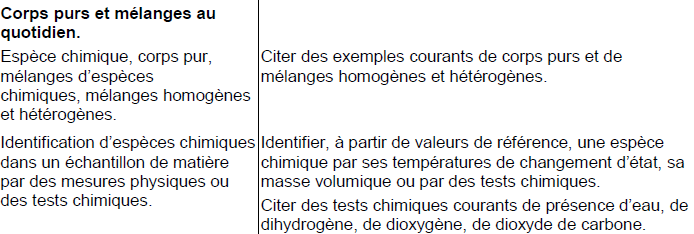
\includegraphics[width=.95\textwidth]{BO1.png}
	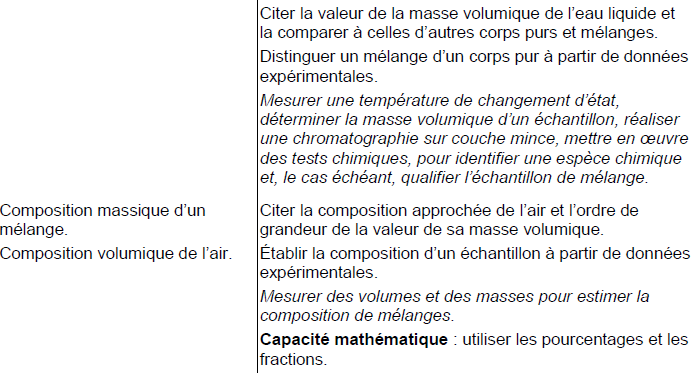
\includegraphics[width=.95\textwidth]{BO2.png}

\end{center}
}


\doc{2}{Exercices dans le livre scolaire}{
		\begin{enumerate}
			\item Compétence de base : exercice 5,6, 9, 10 page 29
			\item Pour confirmer vos compétences : exercice 10, 18 page 29
			\item Parcours expert exercice 20 page 31
		\end{enumerate}
}\vspace{1cm}
	\noindent \textbf{Quiz sur les corps purs et mélanges}
\begin{center}
	\begin{minipage}{.12\textwidth}
		\centering
		
\includegraphics[width=.5\textwidth]{Quiz1.png}
		
		Quiz 1 - Mélanges et corps purs : \url{https://forms.office.com/r/p5gCDE1rn2?origin=lprLink}
	\end{minipage}\hspace{.5cm}
	\begin{minipage}{.12\textwidth}
		\centering
		
\includegraphics[width=.5\textwidth]{Quiz2.png}

		Quiz 2 - Masse volumique: \url{https://forms.office.com/r/NHeZMHKC24?origin=lprLink}
	\end{minipage}\hspace{.5cm}
\begin{minipage}{.12\textwidth}
			\centering
			
\includegraphics[width=.5\textwidth]{Quiz3.png}
	
			Quiz 3 - Identifier des espèces: \url{https://forms.office.com/r/sZqd7qFQ1r?origin=lprLink}
		\end{minipage}
\end{center}


\section*{Introduction}

Quel est le point commun entre de l'huile d'olive, un ordinateur, un chat ou encore l'air que nous respirons ? Les quatre sont composés d'entités chimiques, c'est à dire des atomes, de molécules ou d'ions. Cependant, sont-ils composés d'un seul type d'entités, ou s'agit-il de mélanges ? 

\vspace{-.5cm}
\section{Corps purs et mélanges}

On s'intéresse à la matière à l'échelle \textbf{macroscopique}, c'est à dire à notre échelle. On y observe les composés dans leur globalité.\medskip

Par exemple, étudier un morceau de cuivre\footnote{Le cuivre est un métal de couleur rosée. Les pièces de 1,2 et 5 centimes d'euros en sont recouvertes, d'où leur couleur.} à l'échelle macroscopique consisterait en le peser, mesurer sa température de fusion... En revanche, son étude à l'échelle microscopique impliquerait, par exemple d'identifier les atomes qui le composent.

\begin{definition}{Définition 1 - échelle microscopique}
	En biologie, sciences de la Terre et en physique est microscopique ce qui ne peut être vu qu'à travers un microscope (plus petit que le dixième de millimètre).
\end{definition}


\begin{definition}{Définition 2 - échelle macroscopique}
	En biologie, sciences de la Terre et en physique est macroscopique ce qui peut être vu à l'\oe il nu.
\end{definition}\bigskip

Il est difficile de donner des valeurs à ces tailles, puisqu'elles dépendent bien souvent du contexte (domaine d'étude, discipline,...)

\subsection{Les espèces chimiques}

À l'échelle microscopique, la matière est constituée d'\textbf{entités chimiques} (molécules, atomes, ions).\medskip


\begin{definition}{Définition 3 - Espèce chimique}
Une espèce chimique est un ensemble d'entités chimiques identiques.
\end{definition}

Une espèce chimique est caractérisée par des données telles que sa \textbf{formule chimique}, son nom, son aspect, sa température de fusion, ses propriétés chimiques \dots

\begin{figure}[ht]
	\centering
	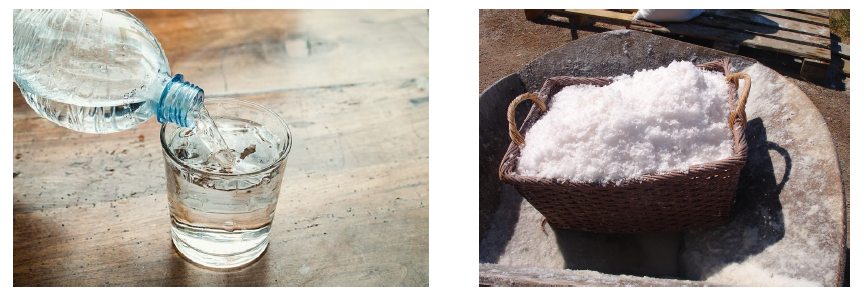
\includegraphics[width=.5\textwidth]{sel.png}
	% 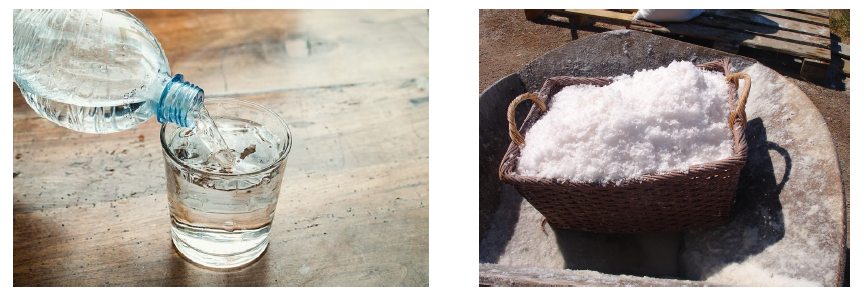
\includegraphics[width=.3\textwidth]{sel.png}
	\caption{À gauche de l'eau, à droite du sel de mer.}
\end{figure}

\exo{1}{Espèce chimiques}{Donner le type (atomique, moléculaire ou ionique) des espèces chimiques suivante : hélium (He), eau ($\rm H_2O$), chlorure de sodium ($\rm Na^+, Cl^-$).\medskip

L'hélium, est un atome, l'eau ($\rm H_2O$) est une molécule, tandis que le chlorure de sodium est un composé ionique. }

\subsection{Corps purs}

\begin{definition}{Définition 4 - Corps pur}
	
Un corps pur est constitué d'une seule espèce chimique.
\end{definition}

On distingue deux types de corps purs : 
\begin{enumerate}
	\item Les corps purs simples composés d'un seul type d'atomes;
	\item Les corps purs composés, qui comportent plusieurs types d'atomes (dans des proportions bien définies pour le corps pur considéré).
\end{enumerate}

\exo{2}{Corps purs}{Indiquer, pour les corps purs suivants, s'il s'agit de corps purs simples ou composés : charbon (C), dioxygène ($\rm O_2$), eau ($\rm H_2O$), éthanol ($\rm C_2H_6O$).\medskip

\noindent \textbf{Solution:}\medskip

Le charbon et le dioxygène sont des corps pur corps pur simple car ils sont constitués chacun d'une seule sorte d'atome. L'eau et l'éthanol sont constitués de corps purs composés car ils sont composés de différents atomes qui restent dans des proportions bien définies. }
\subsection{Les mélanges}

\begin{definition}{Définition 5 - Mélanges}
	Un mélange est constitué de plusieurs espèces chimiques différentes.
\end{definition}

Lorsque l'on mélange plusieurs espèces chimiques, deux types de mélanges peuvent se former:\bigskip

\begin{itemize}
	\item Si le mélange est constitué d'\textbf{une seule phase} (on ne peut plus distinguer à l'\oe il nu les constituants après agitation), on parle de \textbf{mélange homogène};\medskip
	
	\item Dans le cas contraire, il est qualifié de \textbf{mélange hétérogène}.
\end{itemize}

Deux liquides formant un mélange homogène sont dits \textbf{miscibles}.

\exo{3}{Mélanges}{Dire, pour chaque composé ci-dessous, s'il s'agit d'un mélange homogène ou hétérogène.
\begin{center}
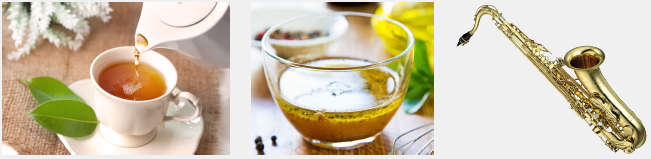
\includegraphics[width=.95\textwidth]{Melanges.png}
\end{center}
\captionof{figure}{De gauche à droite, du thé, une vinaigrette, un saxophone.}
}

% \clearpage
\section{Comment identifier les espèces chimiques}

% Dans cette partie, on s’intéresse à l’identification des espèces chimiques. Cela
% consiste à déterminer la nature d’un composé donné. 
On dispose pour cela de différentes méthodes, physiques comme chimiques.
% \vspace{-.4cm}

\subsection{Méthodes physiques}

\subsubsection{La masse volumique}

Pour identifier une substance, on peut mesurer certaines de ses caractéristiques physiques: aspect, indice de réfraction, température de fusion, masse volumique \dots On détaille ici ces deux derniers points.\medskip

\textbf{La masse volumique} caractérise la masse d'un matériau \textbf{par unité de volume}. Par exemple, la masse volumique du plomb est plus grande que celle de l'eau car 1 m$^3$ de plomb est plus lourd que 1m$^3$ d'eau. En revanche, 20m$^3$ d'eau sont plus lourds (ont une masse plus grande) que 1m$^3$ de plomb.

\begin{figure}[ht]
	\centering
	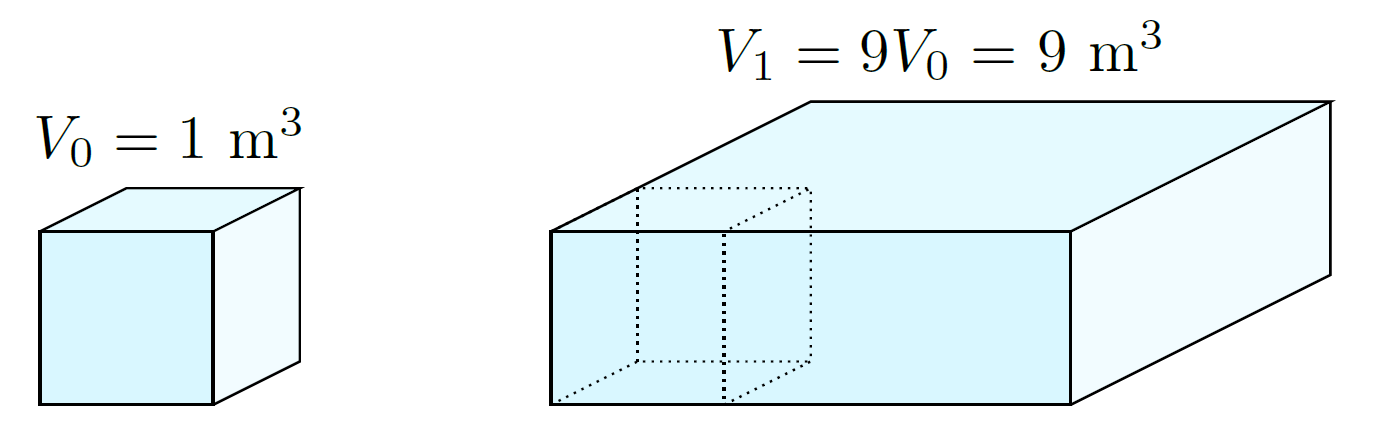
\includegraphics[width=.3\textwidth]{volume.png}
	\caption{À gauche, 1 m$^3$ d’eau pesant 1000 kg. À gauche, 9 m$^3$ pesant 9000 kg. Les masses d’eau sont différentes, mais les masses volumiques sont identiques.}
\end{figure}

\begin{definition}{Définition 6 -  Masse volumique}
	
	La masse volumique $\rho$ \og{}rho\fg{} d'un échantillon de matière est une grandeur égale au quotient de sa masse $m$ par le volume $V$ qu'il occupe. Elle est donc définie par la relation : 
	
	\begin{equation}
		\rho = \dfrac{m}{V}
	\end{equation}

	$\rho$ est donnée en $\rm kg/m^3$, $m$ en kg et $V$ en m$^3$.
\end{definition}
C'est là tout l'intérêt de la masse volumique par rapport à la masse : la masse volumique de 1m$^3$ d'eau est la même que celle de 20m$^3$ d'eau. Ce n'est pas le cas pour leurs masses. 

\begin{Proposition}{Propriété 1 - masse volumique}
	La masse volumique caractérise le matériau \textbf{indépendamment} de la quantité de matière de celui-ci.
\end{Proposition}\medskip

% \begin{minipage}{.5\textwidth}
\begin{definition}{Définition 7 - Densité}
La densité est définie par la relation :
\begin{equation}
	d = \dfrac{\rho}{\rho_{eau}}
\end{equation}

La densité est un nombre sans dimension, donc les masses volumiques doivent être exprimées dans les mêmes dimensions.
\end{definition}

Voici les densités de quelques solvants courants:\smallskip

\begin{table}[ht]
	\centering
	% \resizebox{.2\textwidth}{!}{%
	\begin{tabular}{|c|c|c|}
	\hline
	\rowcolor[HTML]{C0C0C0} 
	\textbf{Nom} & \textbf{Masse volumique  ($\rm kg\cdot m^{-3}$)} & \textbf{Densité} \\ \hline
	Eau          & 1000                                             & 1,0              \\ \hline
	Air          & 1,2                                              & 0,0012           \\ \hline
	Essence      & 680 à 790                                        & 0,68 à 0,79      \\ \hline
	Éthanol      & 790                                              & 0,79             \\ \hline
	Or           & 19300                                            & 19,3             \\ \hline
	\end{tabular}%
	% }
	\end{table}
% \end{minipage}
% \clearpage

	\exo{4}{Masse volumique}{Répondre aux questions suivantes en détaillant votre raisonnement :
	
	\begin{enumerate}
		\item Quelle est la masse d'un litre d'eau ? 
		\item Quel est le volume occupé par 1 kg d'essence ?\vspace{.2cm}
	\end{enumerate}

	\noindent \textbf{Solutions :}\medskip

	1. Par définition $\rho = m/V$ soit $m=\rho \times V$ Par conséquent $m=1000\times 1\times 10^{-3} = 1~\rm kg.$
	
	2. $V = m/\rho$, donc $V = 1/790 \approx 1\times 10^{-3} m^3 = 1~\rm L$
		
	}
\subsubsection{Température de changement d'état}

		On peut également identifier une espèce chimique en mesurant sa \textbf{température de changement d'état}, et en la comparant aux valeurs de référence.

		\begin{figure}[ht]
			\centering
			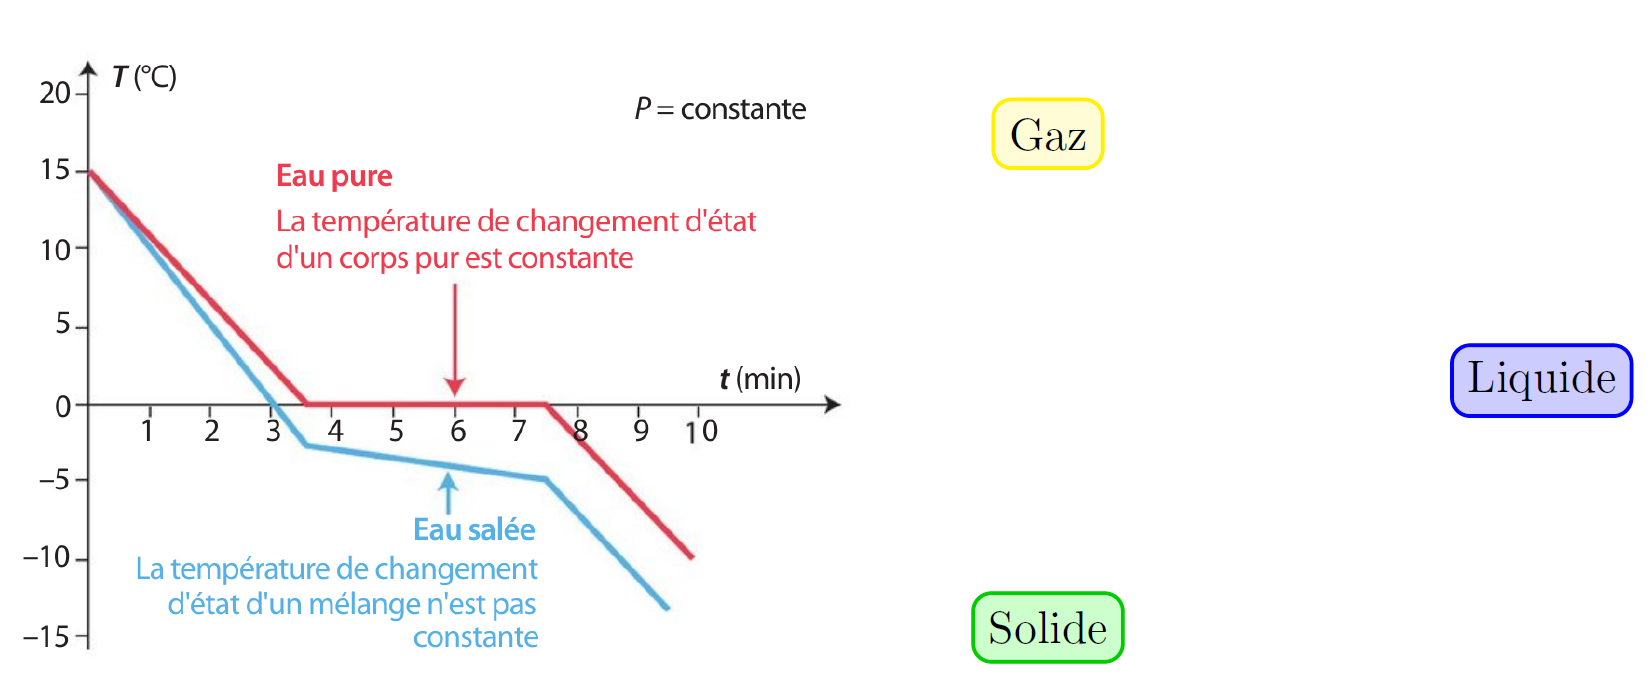
\includegraphics[width=.4\textwidth]{TemperatureChangementDetat.png}
			\caption{Lorsqu'on refroidit de l’eau pure, on observe \textbf{un palier} de température correspondant à la température de fusion de l’eau. Ce n’est pas le cas pour un
			mélange.}
		\end{figure}

		Dans le cas d'un liquide, on peut mesurer une \textbf{température d'ébullition} notée $\theta_{eb}$ (\og{}thêta\fg{}) à l'aide d'un thermomètre. Dans le cas d'un solide, on peut mesurer sa \textbf{température de fusion} notée $\theta_f$ à l'aide d'un \textbf{banc Kofler}. 
		Contrairement aux corps purs, les mélanges n'ont pas de changement d'états définies.
% \clearpage
% \begin{figure}[ht]
% 	\centering
% 	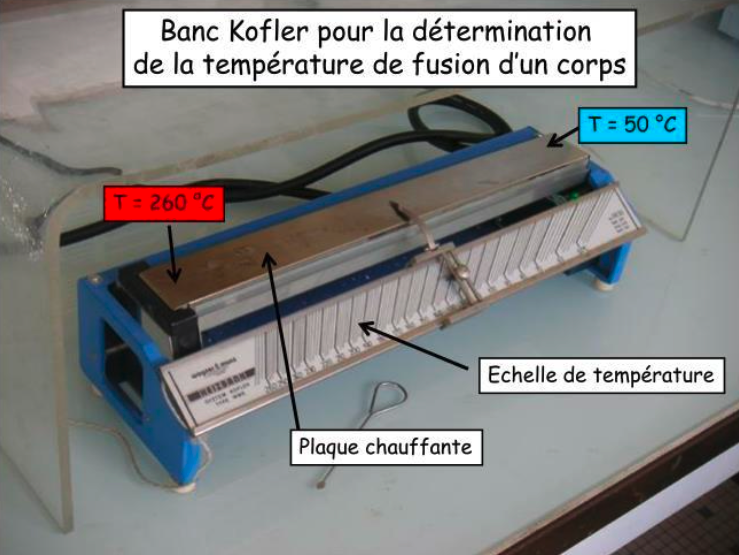
\includegraphics[width=.4\textwidth]{kofler.png}
% 	\caption{Photo d'un banc kofler.}
% \end{figure}

\subsection{La solubilité}

\begin{definition}{Définition 8 - Solubilité}
	\medskip

	La solubilité notée $s$ et exprimée en $~\rm g\cdot L^{-1}$ d'une espèce chimique correspond à la masse maximale de cette espèce que l'on peut dissoudre dans une solution.
\end{definition}
\clearpage


		\subsection{Méthodes chimiques}


		On peut également identifier certaines espèces chimiques par des \textbf{tests chimiques}. On rappelle les plus classiques de ces tests :

		\begin{itemize}
			\item Pour détecter la présence d'eau (formule $\rm H_2O_{(l)}$) dans un mélange, on peut le mettre en contact avec du \textbf{sulfate de cuivre anhydre}
			\begin{figure}[ht]
				\centering
				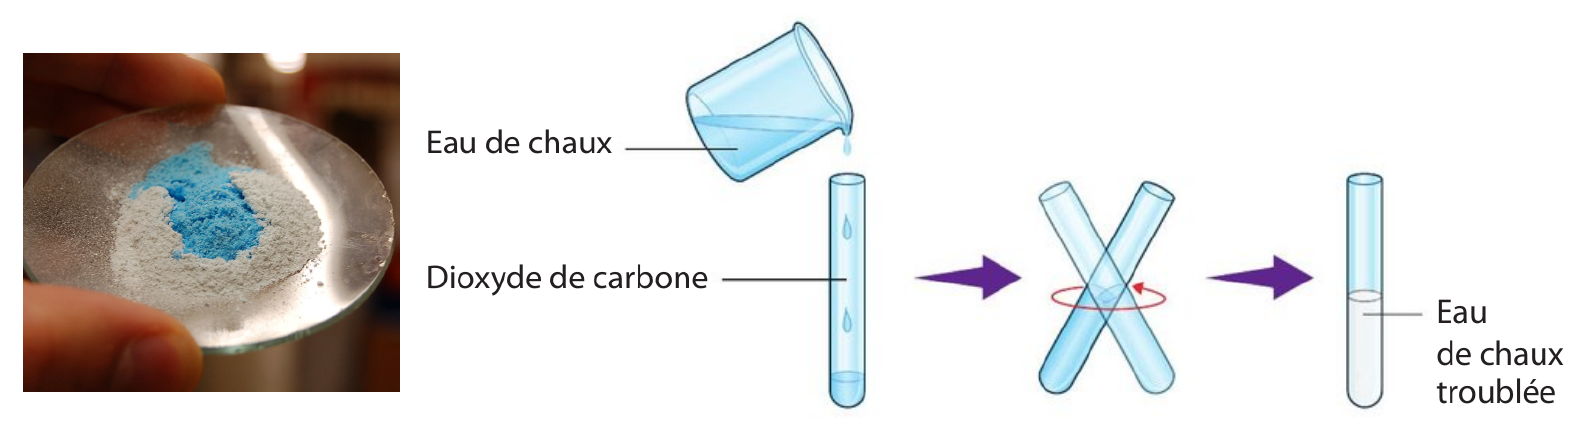
\includegraphics[width=.5\textwidth]{sulfatedecuivre.png}
				\caption{Tests de présence d’eau (gauche) et de dioxyde de carbone (droite).}
			\end{figure}
			% \vspace{2cm}
			\item Pour identifier du \textbf{dioxyde de carbone (de formule ($\rm CO_2(\rm g)$))} dans un gaz, on peut le faire barboter dans de \textbf{l'eau de chaux}, il apparaît alors un léger \textbf{trouble} si le test est positif.
			\item Pour vérifier la présence de \textbf{dioxygène (formule $\rm O_2(g)$)} dans un gaz, on peut approcher une allumette incandescente. Si celle-ci se rallume, du dioxygène est présent.
			\begin{figure}[ht]
				\centering
				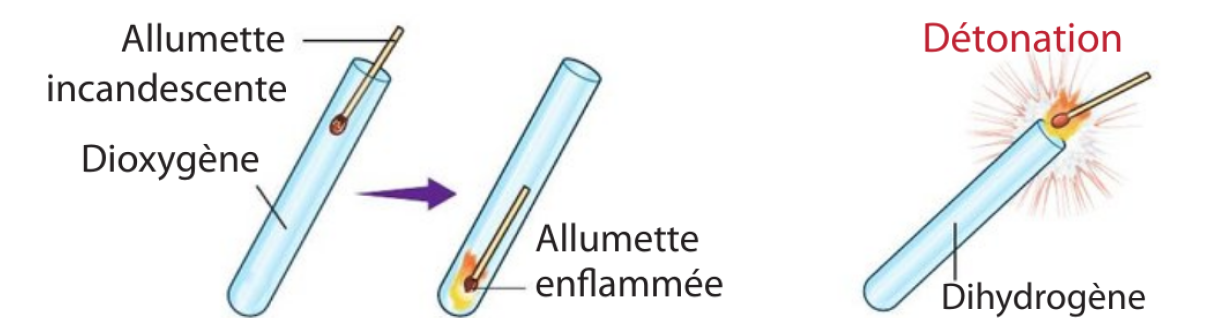
\includegraphics[width=.35\textwidth]{dihydrogène.png}
				\caption{Tests de présence de dioxygène (gauche) et de dihydrogène (droite).}
			\end{figure}

			\item Pour vérifier la présence de \textbf{dihydrogène (formule $\rm H_2(g)$)} dans un tube à essais, on approche une flamme de l'extrémité du tube. Si une petite détonation se produit le gaz contenait du dihydrogène.
		\end{itemize}

		\subsection{Chromatographie sur couche mince}

		\textbf{La Chromatographie sur Couche Mince (CCM} est une méthode permettant de séparer et d'identifier les différentes espèces chimiques présentes dans un mélange. Elle sera étudiée en travaux pratiques.\medskip
		
		Elle consiste à déposer un échantillon d'un mélange sur une plaque en papier ou en silice. Le bas de cette plaque est trempé dans un solvant, qui monte par capillarité, et entraîne avec lui les différentes espèces de l'échantillon.

		\begin{figure}[ht]
			\centering
			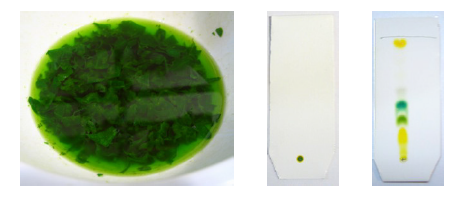
\includegraphics[width=.5\textwidth]{ccm.png}
			\caption{À gauche, mélange de feuilles d’épinard et d’éther diéthylique (qui permet
			d’extraire les chlorophylles). À droite, plaque de chromatographie sur couche mince
			avant et après élution : les différents types de chlorophylle, de couleurs différentes,
			ont été séparés.}
		\end{figure}
% \vspace{-.5cm}
% \clearpage
		\section{Composition d'un mélange}

		Lorsqu'on réalise un mélange, par exemple d'eau et de sucre, il est possible de faire varier la proportion qu'il contient de chacun des corps purs. On peut par exemple réaliser de l'eau peu sucrée, comme très sucrée. La composition massique constitue un moyen de quantifier ces proportions. 
		\vspace{-.5cm}
		\subsection{Pourcentages (rappel mathématique)}

		Le pourcentage permet d'exprimer la proportion des effectifs de deux ensembles présents au sein d'un échantillon sous la forme d'une fraction dont le dénominateur vaut 100. On le note souvent avec le symbole \og{}$\%$\fg{}, ainsi \og{}$\dfrac{70}{100}$\fg{} s'écrit aussi \og{}$70\%$\fg{}.


		\methode{1}{Calcul d'un pourcentage}{Considérons un ensemble contenant $N_R$ boules rouges et $N_B$ boules bleues. Alors le pourcentage $p$ de boules rouges dans l'ensemble s'obtient ainsi : 
		$$p = \dfrac{N_R}{N_B+N_R} = \dfrac{\frac{N_R}{N_B+N_R}\times 100}{100} = \left(\dfrac{N_R}{N_R+N_B}\times 100\right)\%$$}
		
		
		\exo{5}{Pourcentages}{Une urne contient 120 boules vertes et 35 boules jaunes. Calculer le pourcentage de boules jaunes contenues dans cette urne. \medskip
		
		$p_{\rm boules~ jaunes}=\dfrac{N_{jaunes}}{N_{jaunes}+N_{vertes}}=\dfrac{35}{120+35}=0.22 =22\%$
		}



		\subsection{L'air, un mélange de gaz}


		L'air qui nous entour est un mélange de gaz indispensable à la vie. Quand il est sec (c'est à dire sans vapeur d'eau), sa composition en poucentage volumique est d'environ $78\%$ de diazote (formue $N_2$), $21\%$ de dioxygène (formule $\rm O_2$) et $1\%$ d'autres gaz.

		\begin{figure}[ht]
			\centering
			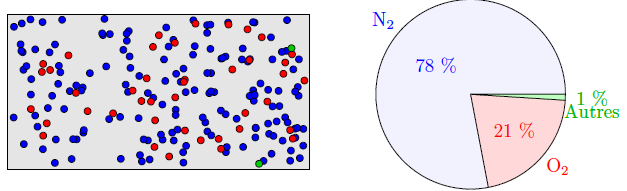
\includegraphics[width=.4\textwidth]{air.png}
			\caption{Représentation schématique d’un échantillon d’air. Les molécules bleues représentent le diazote, les rouges le dioxygène et les vertes l’argon.}
		\end{figure}
Dans les \og{}$1\%$d'autres gaz\fg{}  l'argon est majoritaire. Viennent enseuite des traces de gaz carbonique (formule $\rm CO_2$), de néon, d'hélium,...


		\subsubsection{Fractions massique et volumique}

		Il est commode d'utiliser les pourcentages pour exprimer la composition d'un mélange. La composition massique d'un mélange est déterminée par l'ensemble des fractions massiques de ses constituants. 

		\begin{definition}{Définition 8 - Fraction massique}
			La fraction massique d'un composant est le quotient de la masse du composant "i" et de la masse totale du mélange : 
			\begin{equation}
				w = \dfrac{m_i}{m_{\rm total}}
			\end{equation}
		\end{definition}

		
		\begin{definition}{Définition 8 - Fraction volumique}
			La fraction volumique d'un composant est le quotient du volume du composant "i" et du volume total du mélange : 
			\begin{equation}
				 V_i = \dfrac{v_i}{v_{\rm total}}
			\end{equation}
		\end{definition}

\end{document}

%%
%% FIN DU DOCUMENT
%%
